

% A mathematical optimization problem is generally formulated as:

\begin{sstTitleBox}[Plum]{
		Mathematical Optimization Problem
	}
	\begin{minipage}{0.70\linewidth}
		\begin{sstOnlyFrame}[Plum]
			\textbf{Decision variable} $x  \in \mathbb{R}^{n}$

			\textbf{Objectivce function} $f: \dom(f)\to\mathbb{R}$

			\textbf{Inequality constraints} $g_i$
			$\scriptstyle(i \in \#\text{constraints})$

			\textbf{Equality constraints} $h_i$
			$\scriptstyle(i \in \#\text{constraints})$

			\textbf{Fesabile set}
			$\mathcal{X}\!\!:=\!\!\{x|g(x)\!\!\le\!\!0,\!h(x)\!=\!0\}$
		\end{sstOnlyFrame}
	\end{minipage}
	\begin{minipage}{0.28\linewidth}
		\begin{sstFullFrame}[Plum]
			{\color{white}
				\vspace{-1mm}
				\[ \begin{aligned}
						 & \textbf{minimize }f(x)   \\
						 & \ \ \ \text{subject to:} \\
						 & \ \ \ g_i(x)  \le 0      \\
						 & \ \ \ h_i(x)  = 0
					\end{aligned} \]
				\vspace{-1mm}
			}
		\end{sstFullFrame}
	\end{minipage}

	\begin{sstOnlyFrame}[Plum]
		\textbf{Feasible point}
		$x\in\dom(f)$ with
		$g_i(x)\le 0,\ h_i(x)=0$

		\textbf{Strictly feasible point}
		$x$ with strict inequality
		$g_i(x)<0$

		\textbf{Optimal value}
		$f^\star (\text{or } p^\star)=
			\inf\{f(x)|
			g_i(x)\le0,h_j=0 \}$
		$f^\star=+\infty$: OP infeasible,
		$f^\star=-\infty$: OP unbound below

		\textbf{Optimizer}
		% (is set)
		set:
		$\argmin_{x \in \mathcal{X}} f(x):=
			\{ x\in\mathcal{X}|f(x)=f^\star\}$
	\end{sstOnlyFrame}

	\begin{sstOnlyFrame}[Plum]
		$x^\star$ is a \textbf{Global Minimum} if $f(x^\star)\leq f(x)$

		$x^\star$ is a \textbf{Local Minimum} if
		$\exists\ \epsilon > 0$ s.t.
		$f(x^\star)\leq f(x)$
		$\forall x \in \mathcal{X} \cap B_\epsilon(x^\star)$,
		open ball with center $x^\star$ and radius $\epsilon$
	\end{sstOnlyFrame}
\end{sstTitleBox}


\subsection{Convex Sets, POLYTOPES}

\begin{definition}[Convex Set]
	Set $\mathcal{C}$ is convex if and only if
	\[\theta x + (1-\theta)y \in \mathcal{C},
		\ \forall\ x,y \in \mathcal{C},
		\ \forall\ \theta \in [0,1]\]
\end{definition}


\textbf{Intersection}
$\mathcal{C}_1, \mathcal{C}_2$ cv
$\Rightarrow \mathcal{C}_1 \cap \mathcal{C}_2$ convex \textbf{(cv)}

\textbf{Image under affine map}
$\mathcal{C} \subseteq  \mathbb{R}^{n}$ cv
$\Rightarrow \{Ax+b \mid x \in \mathcal{C} \}$ cv

\textbf{Inverse IoaM}
$\mathcal{C} \subseteq  \mathbb{R}^{m}$ cv
$\Rightarrow \{x\in\mathbb{R}^{n} \mid  Ax+b\in\mathcal{C}\}$ cv

\begin{definition}[Hyperplanes]
	$\{x \in \mathbb{R}^n \mid a\T x=b\}$
\end{definition}
\begin{definition}[Halfspaces]
	$\{x \in \mathbb{R}^n \mid a\T x\le b\}$

	can be \textbf{open} (strict inequality)
	or \textbf{closed} (non-strict inequality)
\end{definition}

\begin{definition}[Polyhedra] intersection of
	\textbf{finite} number of closed halfspaces:
	polyhedra $\{x\in\mathbb{R}^n\mid A^{q\times n}x\preceq b^{q\times1},
		% C^{r\times n}x=d^{r\times1}
		\}$
\end{definition}

\begin{definition}[Polytope]
	is a \textbf{bounded} polyhedron.
\end{definition}

\begin{definition}[Convex hull]
	for  $\{v_1,...,v_k\}\in \mathbb{R}^{d}$ is:

	co$(\{v_1,...,v_k\}):=
		\{ x|x=\sum_{i}\lambda_iv_i,
		\lambda\ge0, \sum_{i}\lambda_i=1 \}$
\end{definition}

\begin{definition}[Ellipsoid]
	set:
	$\{ x | (x\!-\!x_c)^\top A^{-1}(x\!-\!x_c) \leq 1 \}$
	where $x_c$ is center of ellipsoid,
	$A \succ 0$ (i.e. positive definite)
	(Semi-axis lengths are square roots of eigenvalues of $A$)
\end{definition}

\begin{definition}[Norm Ball]
	$B_r(x):=
		\{\xi\in\mathbb{R}^{n}:|\xi-x|_p<r\}$
	where $p$ defines the $l_p$ norm, $p=\{1|2|..|\infty\}$
\end{definition}

%TODO: norm p1,2,...

\begin{theorem}{Minkowski-Weyl}

	The following statements are equivalent
	for $\mathcal{P}\subseteq \mathbb{R}^d$
	% \begin{itemize}[leftmargin=.5mm]
	% \item

	$\mathcal{P}$ is a polytope and there exists
	$A, b$ s.t $\mathcal{P} = \{x \mid Ax \leq b\}$
	% \item

	$\mathcal{P}$ finitely generated,
	$\exists$ finite set $\{v_i\}$ s.t
	$\mathcal{P}=\text{co}(\{v_1,...,v_s\})$
	% \end{itemize}
\end{theorem}

\begin{definition}[Minkowski Sum]
	For $A, B \subset \mathbb{R}^{n}$, the

	\ssthl{ Minkowski Sum } is
	$A \oplus B := \{x + y | x \in A, y \in B\}$
\end{definition}
\[
	[a,b]\oplus[c,d] = [a+c,b+d]
\]

% \includesvg{images/Pontryagin.svg}
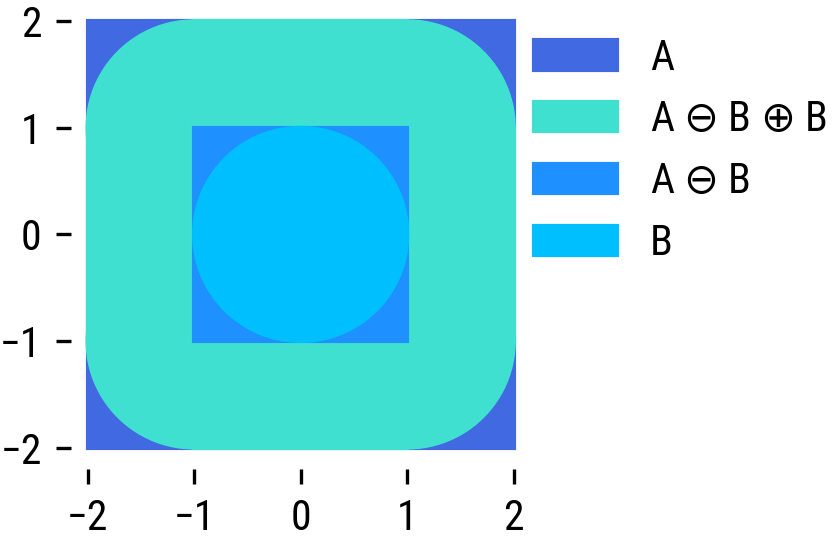
\includegraphics{images/Pontryagin.png}

\begin{definition}[Pontryagin Difference]
	For $A, B \subset \mathbb{R}^{n}$, the
	\ssthl{Pontryagin Difference }is
	$A \ominus B := \{x | x+e \in A, \forall e \in B\}$
\end{definition}
\[
	[a,b]\ominus[c,d] = [a-c,b-d]
\]


%HACK: Polytopic Invariant Set, example e5 Subset test
%Intersection of Polytopes Compute
%Most Common Polytopic constraints? L5.p61

\subsection{Convex Functions}

\begin{definition}[Convex Function]
	$f: \mathcal{C}_\text{convex} \to\mathbb{R}$ is convex iff
	\[
		f(\theta x + (1-\theta)y)\le \theta f(x)+ (1-\theta)f(y),
		\ \forall\ x,y
		\ \forall\ \theta \in [0,1]\]
	$f$ is strictly convex if this inequality is strict.
\end{definition}


\begin{definition}[Epigraph]
	$f:\mathbb{R}^n \rightarrow \mathbb{R}$ cv
	$\Leftrightarrow$
	epi$(f)$ is cv set
	$$\operatorname{epi}(f):=\{(x,t)\in \mathbb{R}^{n+1} | f(x)\le t\}$$
\end{definition}

\textbf{Check Convexity} $f$ is convex if it is
composition of simple convex function
with convexity preserving operations
or if


$f: \mathbb{R}^n \rightarrow \mathbb{R}$ twice differentiable,
$\partial^2f/\partial x^2 \succeq 0\ \forall\ x \in \mathbb{R}^{n}$

$g: \mathbb{R} \rightarrow \mathbb{R}$ with $g(t)=f(x+tv)$
convex in $t\ \forall\ x,v \in \mathbb{R}^{n}$
$\rightarrow f$ convex (restriction to a line)


- the point wise maximum of convex functions is convex

- the sum of convex functions is convex

- $f(Ax+b)$ is convex if $f$ is convex

%NOTE: Level set sublevel set, first, second order convexity



\subsection{Optimality Conditions}

\begin{sstTitleBox}{
		Lagrange Duality
	}
	\begin{centering}
		\vspace{-1.5mm}
		\begin{equation}\text{Consider }
			f^\star = \inf_{x\in\mathcal{\mathbb{R}}^n}f(x)
			\text{ s.t.}\ g(x)\le0,h(x)=0
			\label{eq:dual}
		\end{equation}

		%TODO: Definitions lambda...

		\begin{sstFullFrame}
			{\color{white}
				\vspace{-2mm}
				\[\begin{aligned}
						 & \textbf{Lagrangian}
						 & \hspace{-4mm}	\mathcal{L}(x,\lambda,\nu)
						 & = f(x) + \lambda\T g(x)+\nu\T h(x)
						\\
						\\
						 & \textbf{Dual Function}
						 & \hspace{-4mm}		d(\lambda,\nu)            & = \inf_{x \in \mathcal{\mathbb{R}}^n}\mathcal{L}(x,\lambda,\nu)
					\end{aligned}\]
				\vspace{-2.7mm}
			}
		\end{sstFullFrame}
	\end{centering}
\end{sstTitleBox}

\begin{proposition}[Weak Duality]
	$d(\lambda,\nu)\le f^\star,\forall\lambda\ge0,\nu\in\mathbb{R}^{h}$
\end{proposition}

\begin{definition}[Constraint qualification]
	\textbf{Slater's Condition} holds if $\exists$
	at least one
	\textbf{strictly feasible point}
	$\hat{x}{\ (h(\hat{x})=0,\ g(\hat{x})<0)}$
\end{definition}

\begin{proposition}[Strong Duality]
	If Slater's condition holds
	and OP is convex
	$\Rightarrow$
	$\exists \lambda \ge 0, \nu \in \mathbb{R}^{n_h}$ s.t. $d(\lambda,\nu)=f^\star$
\end{proposition}

\begin{sstTitleBox}[BrickRed]{\textbf{\large
			KKT  Conditions}
		\normalsize(Karush-Kuhn-Tucker)}
	\begin{theorem}[KKT Conditions]
		\begin{centering}
			If Slater's condition holds and
			(\ref{eq:dual}) is convex
			$\rightarrow$
			$x^\star \in \mathbb{R}^{n}$ is a minimizer of the primal (\ref{eq:dual})
			and $(\lambda^\star\ge0,\nu^\star)\in\mathbb{R}^{n_g}\times\mathbb{R}^{n_h}$
			is a maximizer of the dual $\Leftrightarrow$
			is equivalent to the following statements:
			\begin{sstFullFrame}[BrickRed]
				\vspace{-3mm}
				\color{white}
				\small
				\[\begin{aligned}
						\textbf{KKT-1 } & \text{\footnotesize (Stationary Lagrangian)} \hspace{-2mm} &  & \nabla_x\mathcal{L}(x^\star,\lambda^\star,\nu^\star)  =  0
						\\
						\textbf{KKT-2 } & \text{\footnotesize (primal feasibility)}                  &  & g(x^\star)\le0, h(x^\star)                            =                            0
						\\
						\textbf{KKT-3 } & \text{\footnotesize (dual feasibility)}                    &  & \lambda^\star  , \nu^\star \in \mathbb{R}^{n_h}       \ge       0
						\\
						\textbf{KKT-4 } & \text{\footnotesize (complementary}                        &  & \lambda^{\star T} g(x^\star)                          =                          0
						\\
						                & \text{\footnotesize slackness)}                            &  & \nu^{\star T} h(x^\star)                              =  0
					\end{aligned}\]
				\vspace{-4mm}
			\end{sstFullFrame}
			In addition we have:
			$\sup_{\lambda\ge0,\nu\in\mathbb{R}^{n_h}}q(\lambda,\nu)=\inf_{x\in\mathcal{C}}f(x)$
		\end{centering}
	\end{theorem}
\end{sstTitleBox}

\textbf{Remark} Without Slater,
KKT1-4 still implies $x^\star$ minimizes (\ref{eq:dual})
and $\lambda,\nu$ maximizes dual,
but the converse is no longer true.
There can be primal-minimizer/dual-maximizer not satisfy KKT.

%NOTE: Sensitivity Analysis


\subsection{Convex Optimization Problems}

\begin{theorem}
	For a convex optimization problem,
	\textbf{any} locally optimal solution is globally
	optimal (local optima are global optima).
\end{theorem}

\textbf{Linear Programming}
$ \operatorname{minimize} c\T x
	\text{ s.t. } Ax-b \ge 0,\ x\ge0$

Step 1:
$\mathcal{L}(x,\lambda_1,\lambda_2) =
	c\T x-\lambda_1\T (Ax-b) -\lambda_2\T x,\ \lambda_i \ge0$
Step 2:
$\underset{x \in \mathcal{\mathbb{R}}^n}{\operatorname{inf}}
	\mathcal{L}=\lambda_1\T b$
, if $c-A\T\lambda_1-\lambda_2=0$, else $-\infty$

Step 3: Dual,
maximize $b\T\lambda$
s.t.
$c-A\T\lambda\ge0,\lambda\ge0$
(again LP)

\textbf{Quadratic Programming}
min ...

%TODO: LP L3.p40 QP
